\chapter{Het Onderzoek}\label{Het Onderzoek}

Voor deze bachelorproef onderzoek we of we een algemene technieken binnen de machine learning ons een goede analyse van gevoelens kunnen geven op Nederlandse tekst. Verder situeert men zich met het onderzoek  onder supervised learning waarbij we data proberen te classificeren. Zoals eerder vermeldt duidt supervised learning op een gelabelde dataset waar zowel de inputwaarden als de outputwaarde gekend zijn. Concreter hadden we voor het onderzoek de gevoelens veralgemeent tot positief en negatief en een dataset opgebouwd uit reviews van films, muziek en boeken, afkomstig van \url{wwww.moviemeter.nl}, \url{wwww.muziekmeter.nl}
en \url{wwww.boekmeter.nl}.

Het onderzoek is opgedeeld in twee delen. Er is Initi\"eel deel waarbij we de classifiers trainen met een dataset en een onderscheidt maken op basis van de pre-processing techniek. Vervolgens worden de resultaten bekeken op besis van hun precisie. In het tweede deel volgt er een verdere uitdieping van interessante resultaten uit deel \'e\'en.

\section{Initi\"ele onderzoek}\label{Deel 1}

\section{Werkwijze}\label{Werkwijze}

Als hoofddoel willen we te weten komen of het mogelijk is om met algemene technieken uit de machine learning goede classificatieresultaten kunnen behalen. Goede classificatieresultaten uit zich in de precisie waar de classifier met classificeert. In dit onderzoek gaat dit de metriek zijn waarop we bepalen of een classificatie goed of slecht verloopt.\\
We gebruiken de eerder besproken classifiers, namelijk een Naive Bayes classifier en Decission tree als zelflerende algoritmen en trainen Naive bayes classifier telkens met een ander voorbewerkte dataset. De Decission tree trainen we enkel met een LSA voorbewerkte dataset. Als laatste analyseren de telkens de resultaten op basis van de testset en de voorbewerkingstechniek die gebruikt wordt op de dataset.

\section{Resultaten}\label{Resultaten}

Belangrijk om te melden dat volgende resultaten afkomstig zijn door de classifiers te trainen met een moviedataset van 8000 samples, random gekozen, waarvan 6000 trainsamples en 2000 testsamples en dit gemiddeld genomen over 10 runs.
Merk op dat zowel de testset als trainigsset evenwichtig verdeeld zijn.  Dit wil zich dat precies de helft van de set positief is en de andere helft negatief.

Verder wordt er telkens paarsgewijs getest. De testset is altijd hetzelfde voorbewerkt als de trainingsset van de classifier.

Het eerste wat hier is weergegeven, zijn de resultaten van een Naive Bayes Classifier met als trainingsset filmrecensies en als testset film- , muziek en boekrecensies. 

\begin{table}[h]
\centering
\begin{tabular}{|l|l|l|}
\hline
\textbf{Pre-processing techniek} & \textbf{Precisie Trainingsset} &\textbf{Precisie Testset}      \\    \hline
Bag of words     & 86,66\%                        & 58,30\%                       \\    \hline
Remove stopwords & 94,68\%                        & 64,19\%                       \\    \hline
Bigram (n=200)   & 99,26\%                        & 61,75\%                       \\    \hline
Bigram (n=50)    & 94,68\%                        & 64,19\%                       \\    \hline
Best Features + bigram (n = 200) & 94,89\%        & 64,70\%                        \\    \hline
\end{tabular}
\caption{Resultaten van de Naive Bayes Classifier met als trainingsset en testset filmrecensies}
\hspace{2em}
\end{table}

\begin{table}[h]
\centering
\setlength\tabcolsep{4pt}
\begin{minipage}{0.48\textwidth}
\centering
\begin{tabular}{|l|l|}
\hline
\textbf{Pre-processing techniek} & \textbf{Precisie}\\ \hline
Bag of words                     & 53,81\%          \\ \hline
Remove stopwords                 & 60,04\%          \\  \hline
Bigram (n=50)                    & 58,27\%          \\  \hline
Bigram (n=200)                   & 59,75\%          \\  \hline
Best Features                    & 54,94\%          \\  \hline
Best Features + bigram (n = 200) & 61,49\%          \\    \hline
\end{tabular}
\caption{Resultaten van een Naive bayes classifier met een als trainingsset filmrecensies en als testset boekrecensies}
\label{tab:accuracy}
\end{minipage}%
\hfill
\begin{minipage}{0.48\textwidth}
\centering
\begin{tabular}{|l|l|}
\hline
\textbf{Pre-processing techniek} & \textbf{Precisie}\\ \hline
Bag of words                     & 53,17\%          \\ \hline
Remove stopwords                 & 58,18\%          \\ \hline
Bigram (n=50)                    & 56,48\%          \\ \hline
Bigram (n=200)                   & 57,05\%          \\ \hline
Best Features                    & 54,24\%          \\ \hline
Best Features + bigram (n = 200) & 58,72\%          \\    \hline
\end{tabular}
 \caption{Resultaten van een Naive bayes classifier met een als trainingsset filmrecensies en als testset muziekrecensies} 
 \label{tab:ompdiff} 
\end{minipage}
\end{table}

Wat meteen is dat er niet echt een beduidend verschil is tussen de pre-procestechnieken. Ook zien we in tabel 3.BLA dat de beste resultaten worden behaald wanneer de train- en testset van dezelfde soort zijn. \\

Volgende classificatieresultaten komen voort uit de classificatie waarbij de train- en testresultaten telkens voorbewerkt zijn door alle stopwoorden en leestekens te verwijderen. Dan de sets om te vormen naar een tfidf-matrix en tenslotte LSA uit te voeren en ieder document te reduceren naar 2 features.
%
%resultaten lsa voor verschillende models TFIDF , verwijderen van stopwoorden, LSA 
\begin{table}[h]
\centering
\begin{tabular}{|l|l|l|}
\hline
\textbf{Model}              &\textbf{Precisie Trainingsset}    &\textbf{Precisie Testset}    \\   \hline
Decision Tree               & 99,77\%                          & 99,22\%                     \\  \hline
Naive Bayes classifier      & 99,82\%                          & 51,35\%                     \\ \hline 
\end{tabular}
\caption{Resultaten van de classifiers met als trainingsset en testset filmrecensies, beide voorbewerkt door LSA }
\end{table}

Deze resultaten zijn zeer interessant. Er is duidelijk een groot verschil tussen de precisie van de testset voor de Decision Tree en de Naive Bayes classifier. De Naive Bayes classifier kan totaal niets opmaken uit de LSA features die een document voorstellen. Zeker als je weet als men random zou sorteren de precisie 50\%  zou bedragen. Aan de andere hand zijn de resultaten van de decision tree in combinatie met de  lsa features verrassend goed. Met bij een perfecte classificatie kan de decision tree heel goed het onderscheidt maken tussen positieve en negatieve filmrecensies. Wat een veel betere prestatie is, dan de Naive bayes classifier waarbij men hoogste 64,70\% haalde.

Dit resultaat kan men niet negeren er vergt een dieper onderzoek. Wat we  voorlopig weten op basis van de resultaten is:
%
\begin{itemize}
  \item De Naive Bayes Classifier heeft in het algmeen een slechte classificatieprestatie, zowel wanneer train- en testset van dezelfde soort of verschillend zijn.
  \item De classificatie verbetert niet beduidend wanneer men een andere pre-processing techniek gebruikt.
  \item Classificatie aan de hand van LSA features in combinatie met een decision tree classifier levert goede resultaten op wanneer train- en testset van dezelfde soort zijn.
\end{itemize}
\\
Nu we dit weten, bekijken we de combinatie van LSA en de decision tree classifier wat meer in detail. In de uitdieping gaan we bekijken hoe de classificatieresultaten zich verhouden wanneer men een zelfde of verschillende train- en testset gebruikt. Verder gaan we deze resultaten met die van de Naive Bayes Classifier in dezelfde omstandigheden. Als laatste proberen we classificatieresultaten van de decision tree grafisch in kaart te brengen en te kijken waarom het niet of wel goed presteert.   


\section{Uitdieping onderzoek}\label{Deel 2}

Onderstaande tabel geeft alle classicatieresultaten weer, waarbij de kolommen het type van de trainingsset voorstelt en de rijen de testsets.

\begin{table}[h]
\centering
\setlength\tabcolsep{4pt}
\begin{minipage}{0.48\textwidth}
\centering
\begin{tabular}{|l|l|l|l|}
\hline
Testset & Movies  & Muziek  & Boeken  \\  \hline
Movies  & 98,90\% & 44,01\% & 47,56\% \\  \hline
Muziek  & 57,60\% & 98,67\% & 45,93\% \\ \hline
Boeken  & 42,83\% & 51,89\% & 94,32\% \\ \hline
\end{tabular}
\caption{Resultaten van de classificatie met een Decision Tree, getrained op LSA features met verschillende soorten trainings- en testsets}
\label{tab:accuracy}
\end{minipage}%
\hfill
\begin{minipage}{0.48\textwidth}
\centering
\begin{tabular}{|l|l|l|l|}
\hline
Testset & Movies   & Muziek & Boeken         \\ \hline
Movies  & 0.6215   &        &                \\ \hline
Muziek  & 53,165\% &        &                \\ \hline
Boeken  & 53,81\%  &        & 0.693243243243 \\ \hline
\end{tabular}
 \caption{Resultaten van de classificatie van een Naive Bayes Classifier, getrained met verschillende soorten trainings- en testsets volgens Bag 0f Words} 
 \label{tab:ompdiff} 
\end{minipage}
\end{table}

Als we naar de resultaten kijken zien we dat van alle combinaties de classificatieresultaten waarbij de trainingsset en testset hetzelfde zijn, we de beste resultaten verkrijgen.
Verder valt het opnieuw op dat LSA in combinatie met een decision tree uitermate goed presteert, zowel voor de film- als de boek- en muziekrecensies.
De classificaties van testsets, waarbij de trainingsset een ander onderwerp had, presteren voor beide classifiers slecht.


\begin{figure}%
    \centering
    \subfloat{{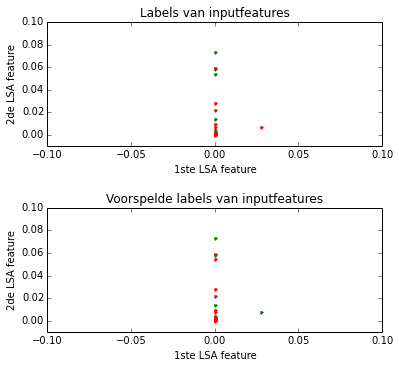
\includegraphics[width=5cm]{resultaten/Trainingsset Boek/Boek/boek-boek-1} }}%
    \subfloat{{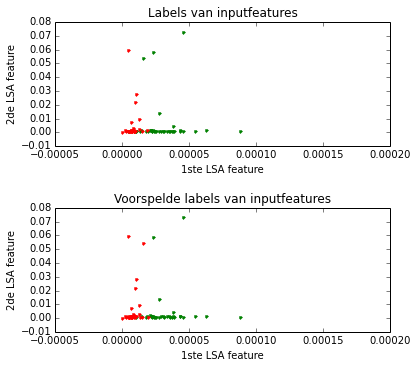
\includegraphics[width=5cm]{resultaten/Trainingsset Boek/Boek/boek-boek-2} }}%
    \subfloat{{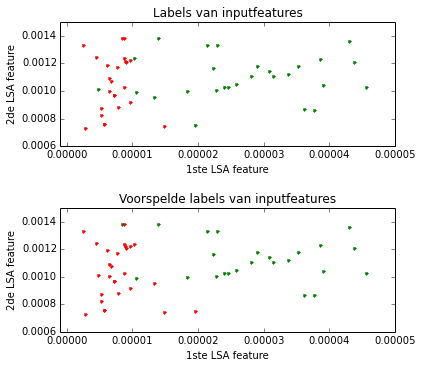
\includegraphics[width=5cm]{resultaten/Trainingsset Boek/Boek/boek-boek-3} }}%
    \caption{Plot van resultaten van de classificatie met een decision Tree, getrained op LSA features met als train- en testset boekrecensies}
    \label{fig:example}%
\end{figure}

\begin{figure}%
    \centering
    \subfloat{{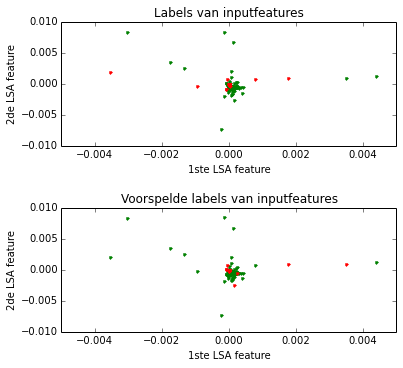
\includegraphics[width=5cm]{resultaten/Trainingsset Movie/Movie/movie-movie-1} }}%
    \subfloat{{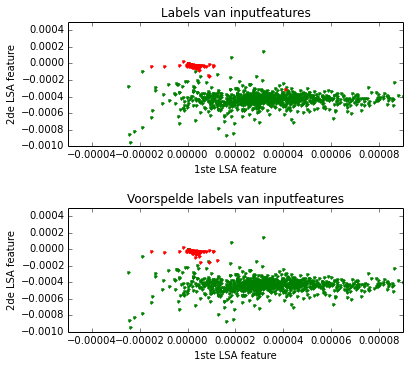
\includegraphics[width=5cm]{resultaten/Trainingsset Movie/Movie/movie-movie-2} }}%
    \subfloat{{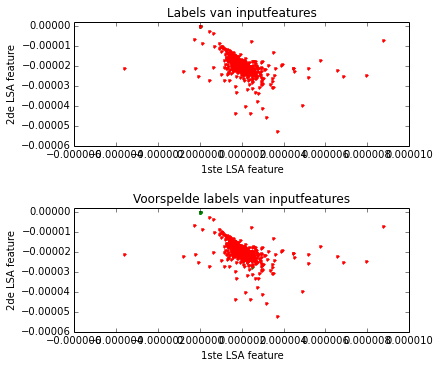
\includegraphics[width=5cm]{resultaten/Trainingsset Movie/Movie/movie-movie-3} }}%
    \caption{Plot van resultaten van de classificatie met een decision Tree, getrained op LSA features met als train- en testset filmrecensies}
    \label{fig:example}%
\end{figure}
%  
\begin{figure}%
    \centering
    \subfloat{{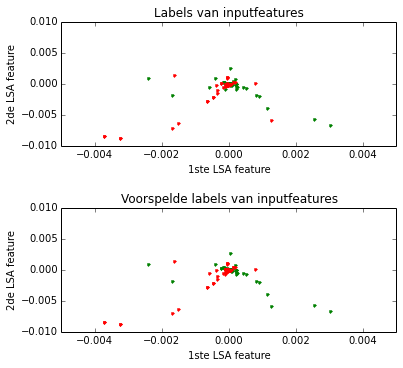
\includegraphics[width=5cm]{resultaten/Trainingsset Muziek/Muziek/muziek-muziek-1} }}%
    \subfloat{{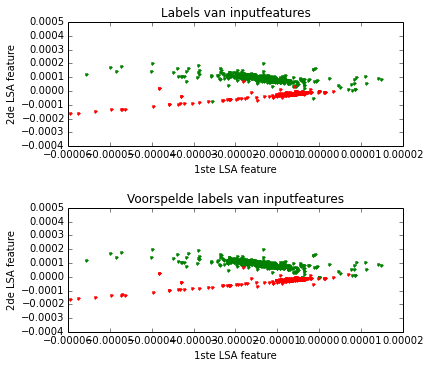
\includegraphics[width=5cm]{resultaten/Trainingsset Muziek/Muziek/muziek-muziek-2} }}%
    \subfloat{{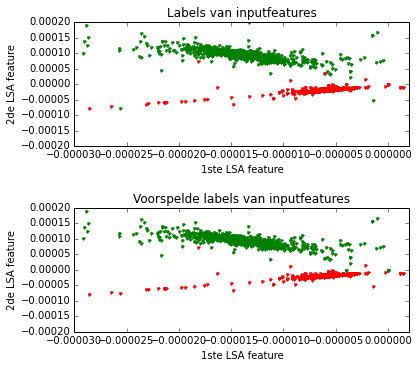
\includegraphics[width=5cm]{resultaten/Trainingsset Muziek/Muziek/muziek-muziek-3} }}%
    \label{fig:example}%
    \caption{Plot van resultaten van de classificatie met een decision Tree, getrained op LSA features met als train- en testset muziekrecensies}
\end{figure}
%  
%andere resultaten 

\begin{figure}%
    \centering
    \subfloat{{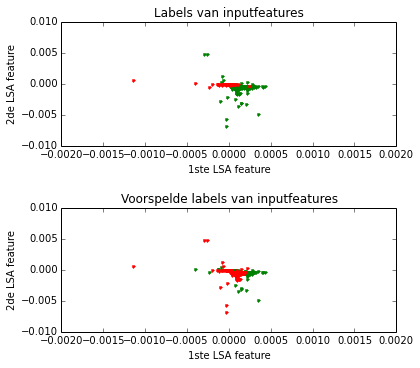
\includegraphics[width=5cm]{resultaten/Trainingsset Muziek/Movie/muziek-movie-1} }}%
    \subfloat{{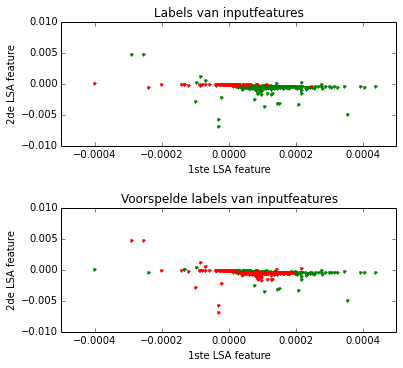
\includegraphics[width=5cm]{resultaten/Trainingsset Muziek/Movie/muziek-movie-2} }}%
    \subfloat{{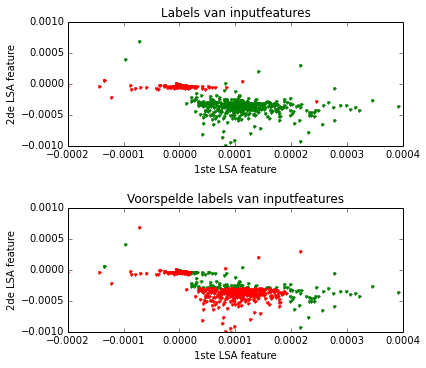
\includegraphics[width=5cm]{resultaten/Trainingsset Muziek/Movie/muziek-movie-3} }}%
    \label{fig:example}%
    \caption{Plot van resultaten van de classificatie met een decision Tree, getrained op LSA features met als trainset muziekrecensies en testset filmrecensies}
\end{figure}
%  

\begin{figure}%
    \centering
    \subfloat{{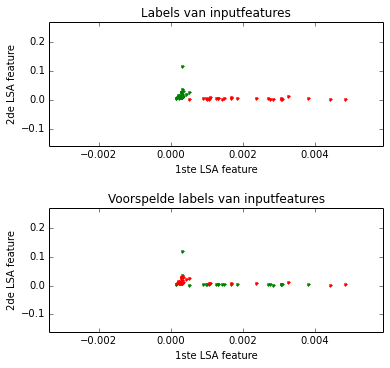
\includegraphics[width=5cm]{resultaten/Trainingsset Muziek/Boek/muziek-boek-1} }}%
    \subfloat{{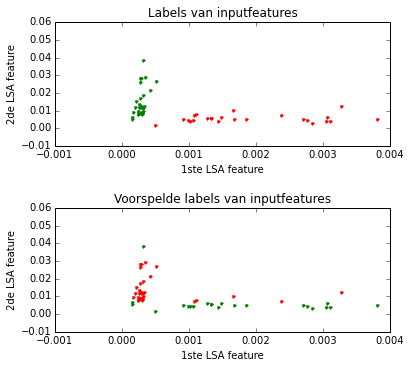
\includegraphics[width=5cm]{resultaten/Trainingsset Muziek/Boek/muziek-boek-2} }}%
    \label{fig:example}%
    \caption{Plot van resultaten van de classificatie met een decision Tree, getrained op LSA features met als trainset muziekrecensies en testset boekrecensies}
\end{figure}
%  

\begin{figure}%
    \centering
    \subfloat{{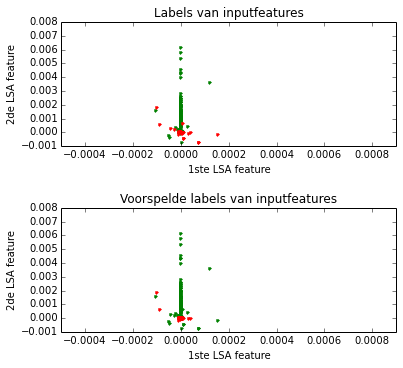
\includegraphics[width=5cm]{resultaten/Trainingsset Movie/Muziek/movie-muziek-1} }}%
    \subfloat{{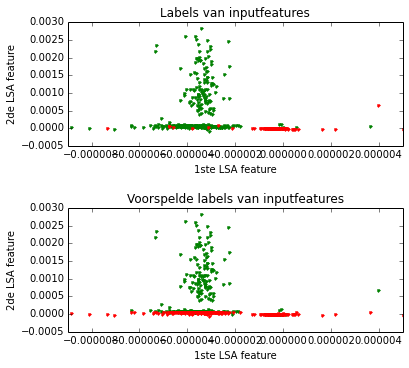
\includegraphics[width=5cm]{resultaten/Trainingsset Movie/Muziek/movie-muziek-2} }}%
     \subfloat{{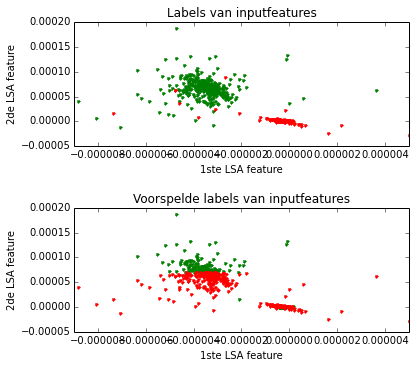
\includegraphics[width=5cm]{resultaten/Trainingsset Movie/Muziek/movie-muziek-3} }}%
     \caption{Plot van resultaten van de classificatie met een decision Tree, getrained op LSA features met als trainset filmrecensies en testset muziekrecensies}
    \label{fig:example}%
\end{figure}
%  
\begin{figure}%
    \centering
    \subfloat{{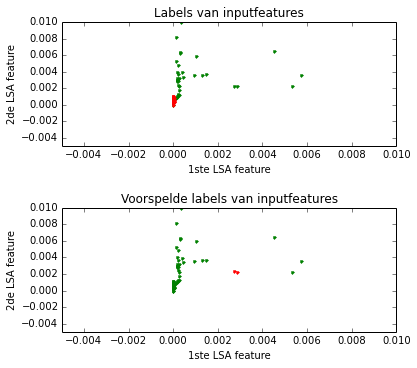
\includegraphics[width=5cm]{resultaten/Trainingsset Movie/Boek/movie-boek-1} }}%
    \subfloat{{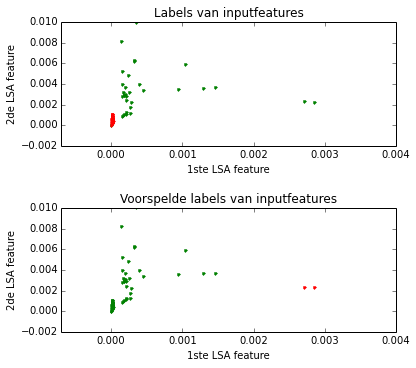
\includegraphics[width=5cm]{resultaten/Trainingsset Movie/Boek/movie-boek-2} }}%
    \subfloat{{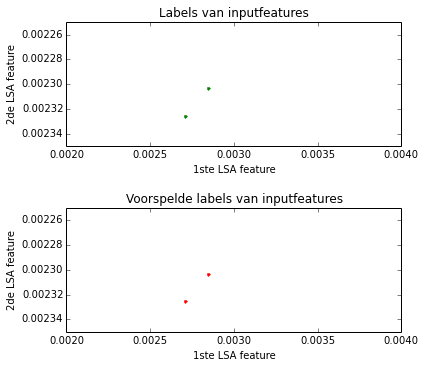
\includegraphics[width=5cm]{resultaten/Trainingsset Movie/Boek/movie-boek-3} }}%
    \caption{Plot van resultaten van de classificatie met een decision Tree, getrained op LSA features met als trainset filmrecensies en testset boekrecensies}
    \label{fig:example}%
\end{figure}
%  

\begin{figure}%
    \centering
    \subfloat{{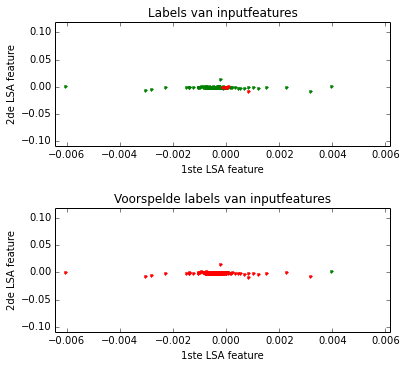
\includegraphics[width=5cm]{resultaten/Trainingsset Boek/Movie/boek-movie-1} }}%
    \subfloat{{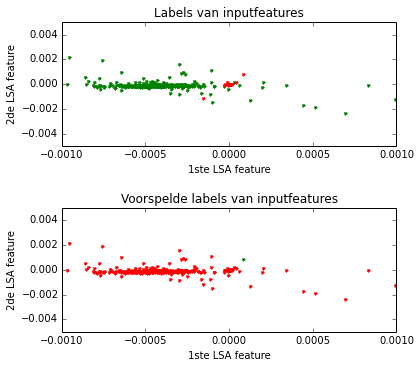
\includegraphics[width=5cm]{resultaten/Trainingsset Boek/Movie/boek-movie-2} }}%
    \subfloat{{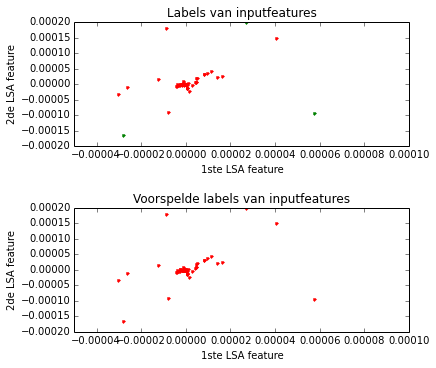
\includegraphics[width=5cm]{resultaten/Trainingsset Boek/Movie/boek-movie-3} }}%
    \caption{Plot van resultaten van de classificatie met een decision Tree, getrained op LSA features met als trainset boekrecensies en testset filmrecensies}
    \label{fig:example}%
\end{figure}
%  

\begin{figure}%
    \centering
    \subfloat{{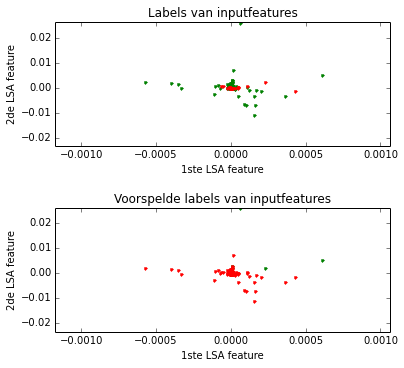
\includegraphics[width=5cm]{resultaten/Trainingsset Boek/Muziek/boek-muziek-1} }}%
    \subfloat{{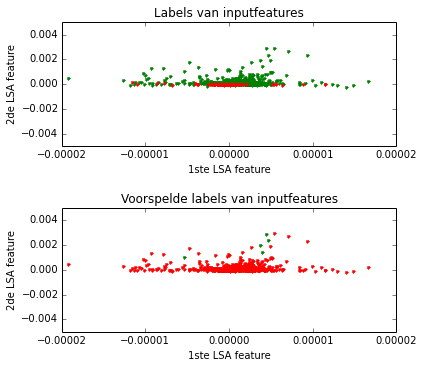
\includegraphics[width=5cm]{resultaten/Trainingsset Boek/Muziek/boek-muziek-2} }}%
    \subfloat{{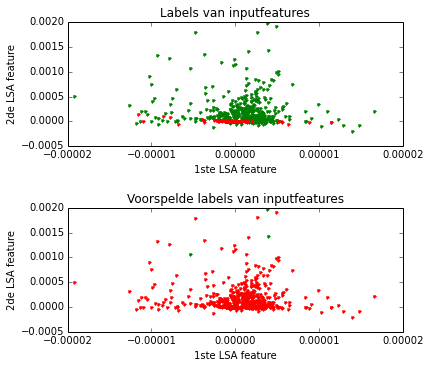
\includegraphics[width=5cm]{resultaten/Trainingsset Boek/Muziek/boek-muziek-3} }}%
    \caption{Plot van resultaten van de classificatie met een decision Tree, getrained op LSA features met als trainset boekrecensies en testset muziekrecensies}
    \label{fig:example}%
\end{figure}
%  

\begin{figure}%
    \centering
    \subfloat{{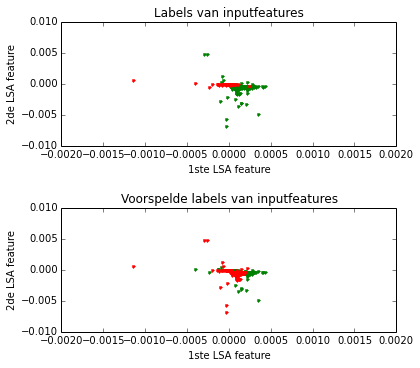
\includegraphics[width=5cm]{resultaten/Trainingsset Muziek/Movie/muziek-movie-1} }}%
    \subfloat{{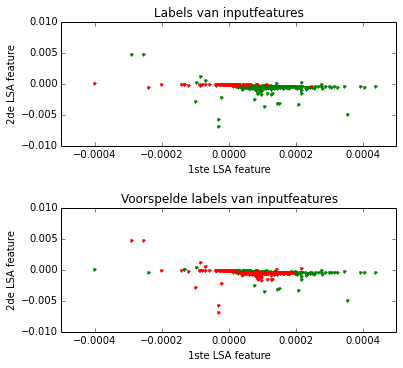
\includegraphics[width=5cm]{resultaten/Trainingsset Muziek/Movie/muziek-movie-2} }}%
    \subfloat{{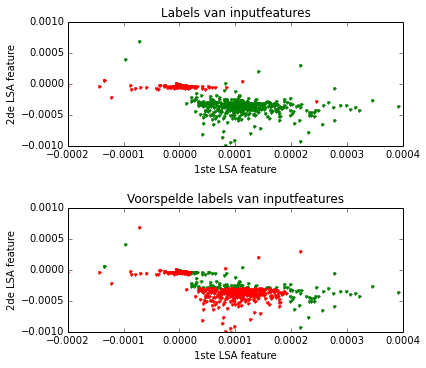
\includegraphics[width=5cm]{resultaten/Trainingsset Muziek/Movie/muziek-movie-3} }}%
    \caption{Plot van resultaten van de classificatie met een decision Tree, getrained op LSA features met als trainset muziekrecensies en testset filmrecensies}
    \label{fig:example}%
\end{figure}
%  





